% Chapter 5

\chapter{SYSTEM DEVELOPMENT} % Write in your own chapter title

\section{Input and Output to System}
\subsection{Input}
Input to the system consists of sensor data by the IMU, JSON-encoded orientation data from the app and images taken by the RPi camera to the quadcopter.
\subsection{Output}
The output of the system consists of automatic stabilization of the quadcopter's flight, change in orientation of the quadcoper and image processing functions respectively.
\newline
1) An upward swipe on the left joystick results in increase in altitude of the quadcopter\newline
2) A downward swipe on the left joystick results in decrease in altitude of the quadcopter\newline
3) An upward swipe on the right joystick results in the quadcopter pitching forward i.e. increase in the back motors\newline
4) A downward swipe on the right joystick results in the quadcopter pitching backward i.e. increase in the front motors\newline
5) An swipe right on the right joystick results in the quadcopter pitching right i.e. increase in the left motors\newline
6) An swipe left on the right joystick results in the quadcopter pitching left i.e. increase in the right motors\newline
\section{Input and Output for each module}
\subsection{Raspberry Pi-controlled quadcopter}
\noindent
\textbf{Input}\newline
The input to Raspberry Pi is the gesture packets from the internet.\newline
1. IMU sensor-data from the accelerometer and gyroscope regrading acceleration and angular velocity.\newline
2. JSON-encoded orientation data from the Android app.\newline
3. JSON-encoded image-acquisition signal data from the Android App.\newline
\newline
\textbf{Output}\newline
There are 3 kinds of outputs based on the input to the quadcopter.\newline
1. IMU sensor data is used ny the PID algorithm to calculate the required orientation and stabilize the quad automatically.\newline
2. Orientation (x,y, z) data is sent to the quad to make it move to the left/right or increase/decrease in altitude.\newline
3. Image acquisition signals allow the RPi camera to click pictures and store them.\newline
\newline
\textbf{Process}\newline
\textbf{Code for Python Server}\newline
\begin{lstlisting}
s = socket.socket()       
host = '0.0.0.0'      
port = 12345          
s.bind((host, port)) 
s.listen(5)          
c, addr = s.accept() 
print 'Got connection from', addr
bus = smbus.SMBus(1)
 while True:
  try:
    msg=c.recv(1024)
    data = json.loads(msg)
    if 'reset' in data:
      quadcopter.set_zero_angle()
      continue
    p = int(data['P'])
    i = int(data['I'])
    d = int(data['D'])
    height = int(data['pitch'])
    quadcopter.set_height(height)
    quadcopter.set_PID(p,i,d)
    except Exception as e:
      print e
quadcopter.stop()
c.close()      
\end{lstlisting} 
\textbf{Code for Balancing the Quad using PID}\newline
\begin{lstlisting}
while self.running:
            start_time = time.time()
            old_pitch, old_roll, old_yaw = pitch, roll, yaw
            (pitch, roll, yaw) = self.imu.read_pitch_roll_yaw()
            (_, _, gx, gy, _, ax, ay, _) = self.imu.read_all()
            axis_output = {'x': 0, 'y': 0, 'z': 0}
            [axis_output['x'],i_x]=self.compute_PID_output(self.kp_x, self.ki_x, self.kd_x, pitch-self.offset_x, i_x, old_pitch)
            [axis_output['y'],i_y]=self.compute_PID_output(self.kp_y, self.ki_y, self.kd_x, roll-self.offset_y, i_y, old_roll)
            [axis_output['z'],i_z]=self.compute_PID_output(self.kp_z, self.ki_z, self.kd_x, yaw-self.offset_z, i_z, old_yaw)
            self.motor_bl.setW(int(self.height+axis_output['x']/2
              +axis_output['y']/2))
            self.motor_br.setW(int(self.height+axis_output['x']/2
              -axis_output['y']/2))
            self.motor_fl.setW(int(self.height-axis_output['x']/2
              +axis_output['y']/2))
            self.motor_fr.setW(int(self.height-axis_output['x']/2
              -axis_output['y']/2))
            end_time = time.time()
            print end_time-start_time
            while(end_time-start_time <= 0.02):
                end_time = time.time()
                time.sleep(0.0001)
            i=i+1
\end{lstlisting} 
\subsection{Image-Processing Module}
\noindent
This module is split into two parts:\newline
1. Panorama stitching\newline
2. 3D Model Reconstruction\newline
\newline
\textbf{Input - Panorama Stitching}\newline
The input consists of images taken by the RPi camera.\newline
\newline
\textbf{Output}\newline
The input images are stitched together forming a 360 degree equirectangular panorama image.\newline
\newline \newline
\textbf{Process}
\begin{lstlisting}
  image_1 = imread(path_to_image_1)
  image_2 = imread(path_to_image_2)

  (keypoints1, descriptors1) = detect_and_compute(image_1)
  (keypoints2, descriptors2) = detect_and_compute(image_2)
  matches = knn(descriptors1,descriptors2)
  points1 = new Array(keypoints1[i] for (i,j) in matches)
  points2 = new Array(keypoints2[j] for (i,j) in matches)
  homography = find_homography(points1,points2)
  (size, offset) = calculate_size(image_1, image_2, homography)
  warped_image = warp_perspective(image_2,homography)
  panorama = warped_image
  panorama[offset_x:offset_x+image_1_width,offset_y:offset_y+image_1_height] = image_1
\end{lstlisting}
\textbf{Input - 3D Reconstruction}\newline
The input consists of images taken by the RPi camera.\newline \newline
\textbf{Output}\newline
Sparse point-cloud representing 3D model of the images taken by the quadcopter rendered on a browser.\newline \newline
\textbf{Process}
\begin{lstlisting}
images = read_images(image_path)
for each image in images:
  features = detect_features(image)
  save_features(features)
matches = {}
for each image1 in images:
  for each image2 in images:
    if image1 not equal to image2:
      count = match_features(image1.features,image1.features)
      if count > threshold:
        matches[image1] = image2
        for each image1 in matches:
          for match in matches[image1]:
            track = add_track(image1,image2)
            create_track_graph(track)
            im1, im2 = find_images_with_largest_matches(images)
            pts3d = bootstrap_reconstruction(im1,im2)
            for each image in images:
              if image not equal to im1 and if image not equal to im2:
                pts2d = get_keypoints(im2)
                pts3d = incremental_reconstruction(pts3d,pts2d)
                pts3d = bundle_adjustment(pts3d)
\end{lstlisting}

\subsection{Android App Module}
\noindent
\textbf{Input}\newline
Touch and click (Haptic) controlled movements on the virtual joystick interface of the app. \newline \newline
\textbf{Output}\newline
Touch movement on the circular joystick results in change in orientation of the quad.
Clicking the camera button send a signal to the RPi Camera to take pictures.
\newline  \newline
\textbf{Process}
\begin{lstlisting}
joystick_left = new Joystick()
joystick_right = new Joystick()
joystick_left.setTouchListener()
joystick_right.setTouchListener()
camera_button.setClickListener()

camera_button.click(){
  camera.shoot()
  camera.enable()
}

while(app_running)
{
  action_left = joystick_left.touch()
  action_right = joystick_right.touch()
  distance_left = joystick_left.getDistance()
  distance_right = joystick_right.getDistance()
  switch(action_left)
  {
    case 'up': increase_height(distance_left)
               break
    case 'down': decrease_height(distance_left)
               break
    default: print 'Invalid action'
  }
  switch(action_right)
  {
    case 'up': pitch_forward(distance_right)
               break
    case 'down': pitch_backward(distance_right)
                 break
    case 'left': pitch_left(distance_right)
                 break
    case 'right': pitch_right(distance_right)
                  break
    case 'upleft': pitch_upleft(distance_right)
                   break
    case 'upright': pitch_upright(distance_right)
                    break
    case 'downleft': pitch_downleft(distance_right)
                     break
    case 'downright': pitch_downright(distance_right)
                      break
    default: print 'Invalid action'
  }
}
\end{lstlisting}


\section{Modules}
\subsection{Raspberry Pi 2-controlled quadcopter}
The objective of the project was to build a semi-autonomous quadcopter capable of self-controlled, stable flight guided via wireless communication through an Android app. 
A quadcopter, also called a quadrotor helicopter or quadrotor, is a multirotor helicopter that is lifted and propelled by four rotors. Quadcopters differ from conventional helicopters as they use rotors which vary the pitch of their blades dynamically as they move around the rotor hub. 
\newline \newline
In the early days of flight, quadcopters were seen as possible solutions to some of the persistent problems in vertical flight; torque-induced control issues as well as efficiency issues originating from the tail rotor could be eliminated by counter-rotation of the relatively short blades which were also much easier to construct.
\newline
\newline
The quadcopter utilizes a Raspberry Pi microcomputer that runs a Python server and takes care of all the on-board computation. It also holds an ESC, IMU sensor and a Raspberry Pi native camera.
\newline \newline
 The Raspberry Pi interfaces with the IMU using an I2C interface that allows it to communicate with the accelerometers, gyroscopes and magnetometers independently using only 2 pins(viz. SCL and SDA pins) by using separate addresses for each. The Pi gets the accelerometer and gyroscope angles separately for each axis and computes on them to find out the overall orientation of the quadcopter.
\newline
\newline
The Raspberry Pi can only supply digital signals that is 0 or 1 i.e. on or off. This does not allow us to directly control the motors to vary their speed. The Electronic Speed Controller (ESC) allows such digital signals to be converted to variable voltage and allow speed regulation of motors by supplying a PWM signal to them. PWM signals are achieved by sending pulses at a certain frequency while controlling the amount of time the pulse is on in a cycle. The longer the pulse is high during a cycle, the higher the voltage supplied to the motor. 
\newline
The ESC also allows an external power souce such as a battery to be used for powering the motors. Our drone uses a 10V LiPo battery. LiPo batteries are commonly used for powering drones because they have high discharge rates required to power the four motors functioning at high speed and requiring order of 20A of current. 
\newline
\newline
The quadcopter's flight is controlled using a PID controller. The PID algorithm is a closed-loop feedback mechanism that is used in control systems. The controller attempts to minimize the error by adjusting control inputs(P,I,D values). In the quadcopter, the PID controller will be taking data measured by the IMU sensor and comparing that against expected values to alter the speed of the motors to compensate for any differences and maintain balance. It involves three separate constant parameters viz. the proportional(P), the integral(I) and derivative(D) values. Heuristically, these values can be interpreted in terms of time: P depends on the present error, I on the accumulation of past errors and D is a prediction of future errors, based on current rate of change.
\newline
\newline
The Proportional Gain Coefficient(P) is the most important value. This coefficient determines which value is more important - those measured by the gyroscopes or those defined by human control. The higher the coefficient, the more sensitive the quadcopter becomes to angular change. If 'P' is too high, the quadcopter will start to oscillate. 
\newline
\newline
The Integral Gain Coefficient(I) is used to increase precision of angular position. This term is extremely useful for combating turbulence due to wind and motors. If this value becomes too high, the reaction speed of the drone will decrease.
\newline
\newline
The Derivative Gain Coefficient(D) is used to allow the quadcopter to reach the desired altitude more quickly as it amplifies the user input. It is dangerous to increase this value as the quadcopter may become highly susceptible to small changes.
\newline
\newline
The quadcopter flight and on-board operations are controlled via WiFi using an Android app. It receives signals encoded as JSON objects as steady stream from the App. The signal carries altitude, trims, motor speeds and camera information to the RPi. The signal is received by a Python server running on the RPi which is decoded and fed as input to the Quadcopter program.  
\newline
\newline
The quadcopter also houses a native Pi camera module which has the ability to take high quality photos and videos. It interfaces with the Raspberry Pi using a Camera Serial Interface. 
\newline
The function of the quadcopter is to take pictures and perform two major image-processing operations viz. Panorama Stitching and 3D-Model Reconstruction.
\newline
The quadcopter itself is small enough to control its flight and large enough to hold all the on-board equipment.
\begin{figure}[H]
  \centering
  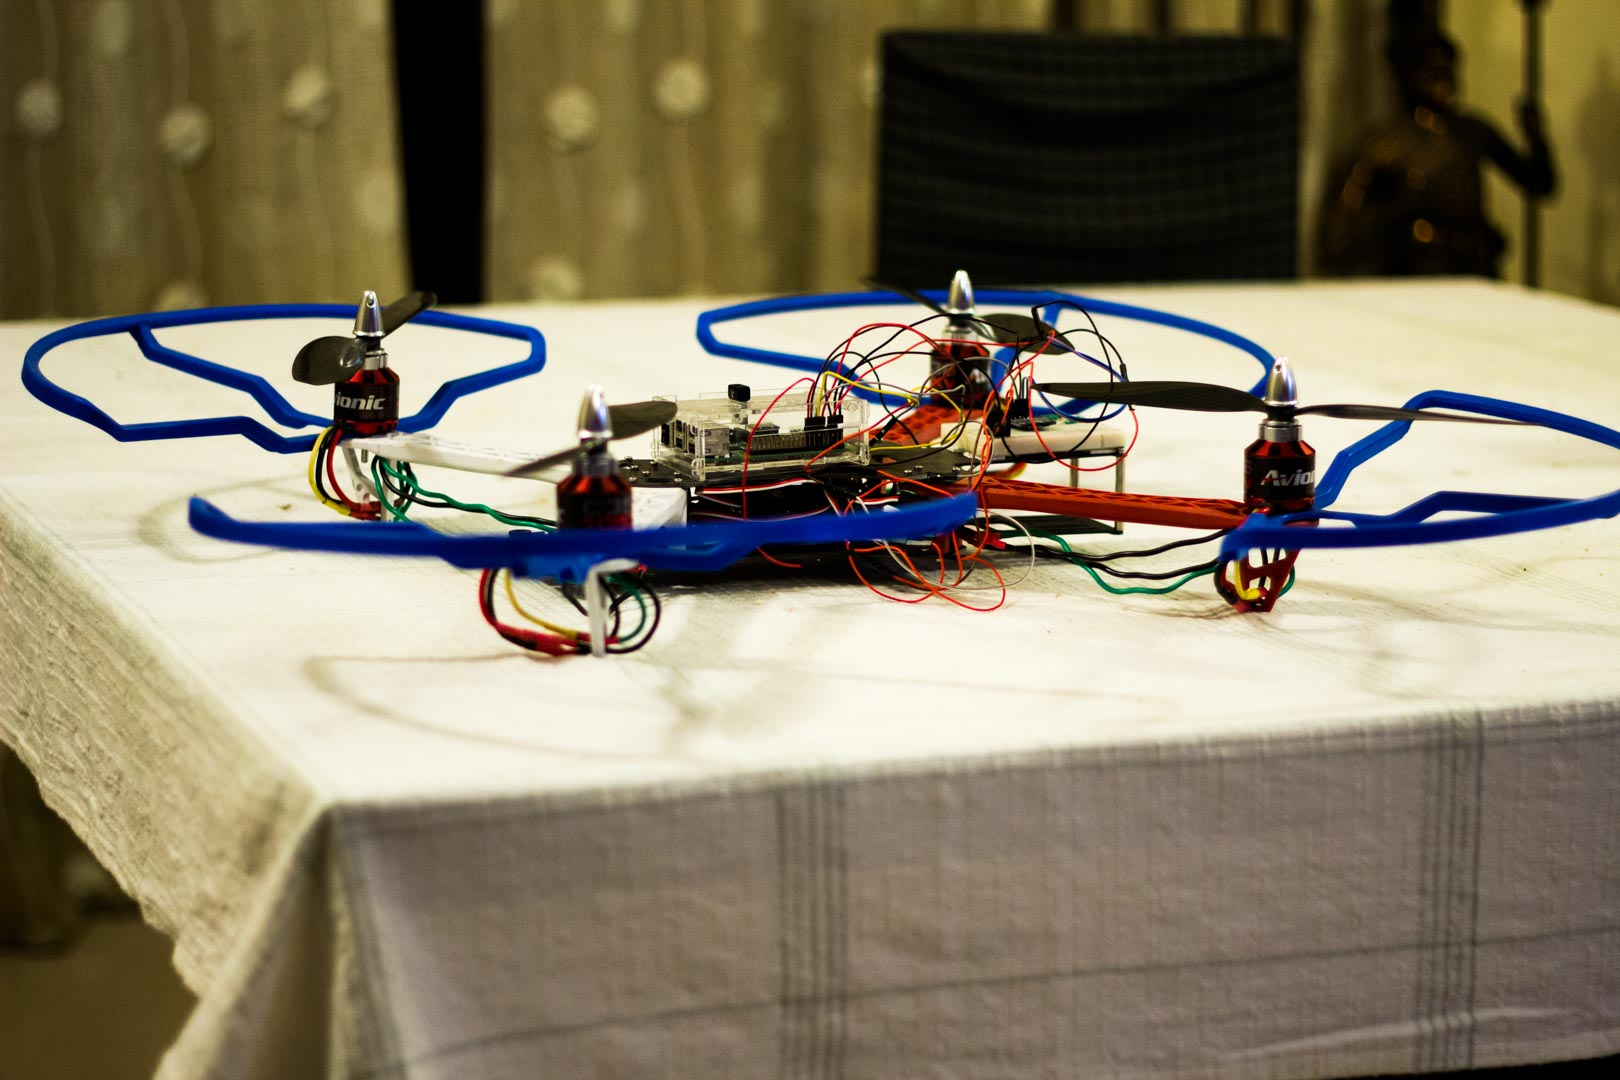
\includegraphics[height = 10cm]{Quad.jpg}
  \caption{The Preliminary Quadcopter without the camera. It carries the ESC, IMU sensor and the RPi. It also has 4 propeller guards (blue) to protect the propellers from excessive damage. }
  \label{first quadcopter}	
\end{figure}

\begin{figure}[H]
  \centering
  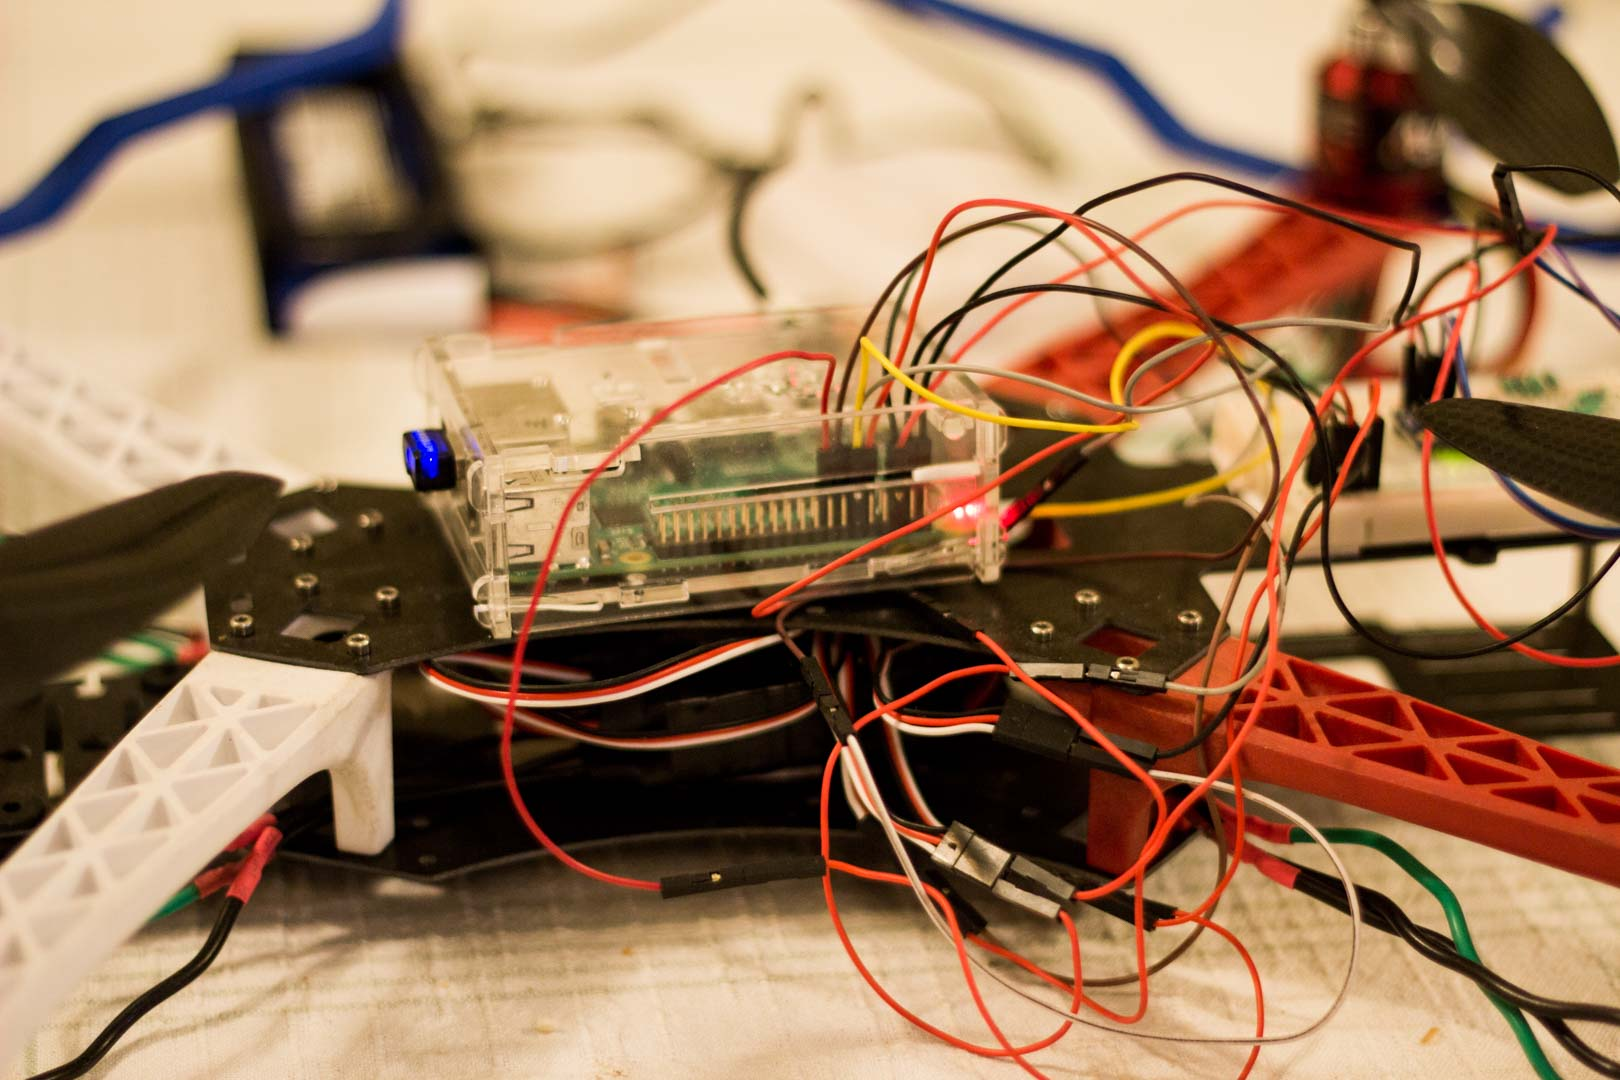
\includegraphics[height = 10cm]{Wiring.jpg}
  \caption{Closer look at the wiring of the quadcopter}
  \label{second quadcopter}	
\end{figure}

\subsection{Image-Processing Module}
The objective of the project is to build a quadcopter that can perform Panorama Stitching and 3D Reconstruction of images taken during its flight. The reason we chose these functions is because the drone is mobile and can capture pictures of inaccessible locations like tall buildings and can perform mapping of wide-open spaces.\newline
 OpenCV is an open-source image processing library which has an enormous number of functionally-rich libraries and detailed online documentation. OpenCV  Version 3.1.0 (the latest version) is used to provide image-processing support in this project.
\newline
\newline
The image-processing module is divided into two parts – Stitching and Reconstruction. The initial stages are the same for both the operations i.e. Acquisition of images, Detecting Features and Matching Features. Feature detection is accomplished using SURF (Speeded Up Robust Features  algorithm and Feature Matching is done by building Kd-Trees and using (K-Nearest Neighbours) Flann Algorithm. Feature detection yields keypoints and descriptors used for matching images.
\newline
\newline
In panorama stitching, RANSAC (Random Sample Consensus) is used to detect outliers and construct a homography matrix. This is essential as it relates pixel coordinates in each pair of images. It is then used to warp the images and construct the panorama by aligning them.
A multi-threaded stitching algorithm has been implemented that stitches images in parallel, reducing the time while maintaining the quality of the constructed image. The quality of the panorama is improved if images are taken with large overlapping features.
\newline
\newline
 3D-Reconstruction is implemented by using the Structure from Motion(SfM) algorithm. The preliminary stage is to calibrate the RPi Camera and calculate intrinsic and extrinsic camera paramaters. Once camera calibration is complete, the images have to be preprocessed to collect metadata i.e. EXIF tags which hold important GPS, latitude, longitude and camera information. 
\newline
\newline
 The next stages are the feature detection and matching stages which have been described above. Matching features are then organized into tracks and a bipartite graph of these 'good tracks' is constructed. This is used to find common tracks and construct the 3D point cloud incrementally. Reconstruction begins with 'bootstrap reconstruction' using two images. The reconstruction consists of triangulating the 2D points to 3D points which is visualized as a point cloud. Consequently, the rest of the images' points are added incrementally to the point cloud. 
\newline
\newline
 After each addition, Bundle Adjustment is done to minimize the reprojection error. Once all the images have been added to the reconstruction, the final point cloud is generated and stored as a '.ply' file. The point cloud is visualized in an interactive browser environment using a Javascript Library called, 'threeJS'.

\begin{figure}[H]
  \centering
  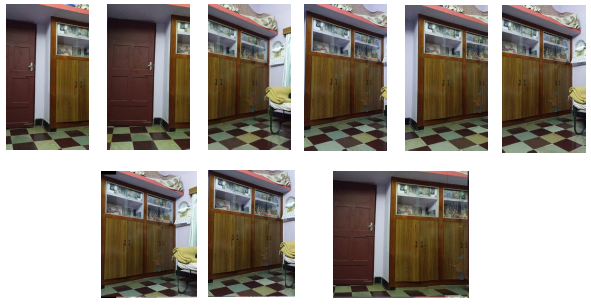
\includegraphics[width = 11cm]{pano.png}
  \caption{Incremental panorama stitching of test images}
  \label{pano}	
\end{figure}

\begin{figure}[H]
  \centering
  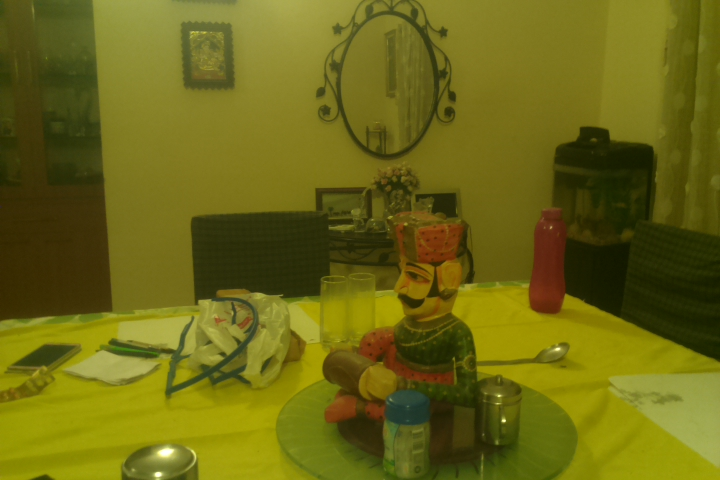
\includegraphics[width = 2.6cm]{pano3d/3d1.jpg}
  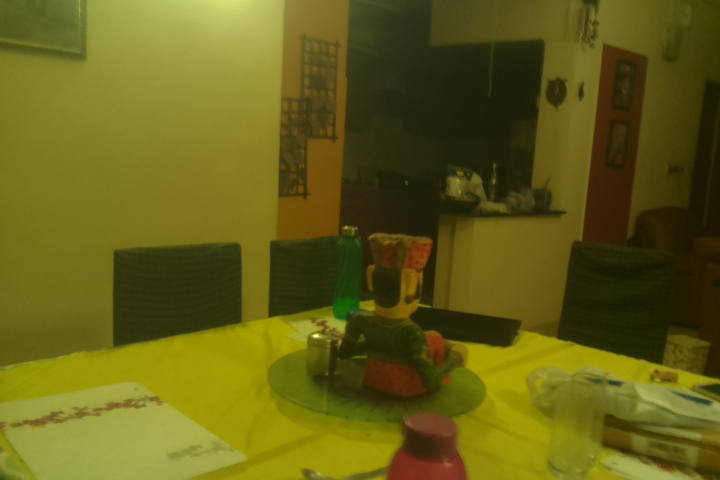
\includegraphics[width = 2.6cm]{pano3d/3d2.jpg}
  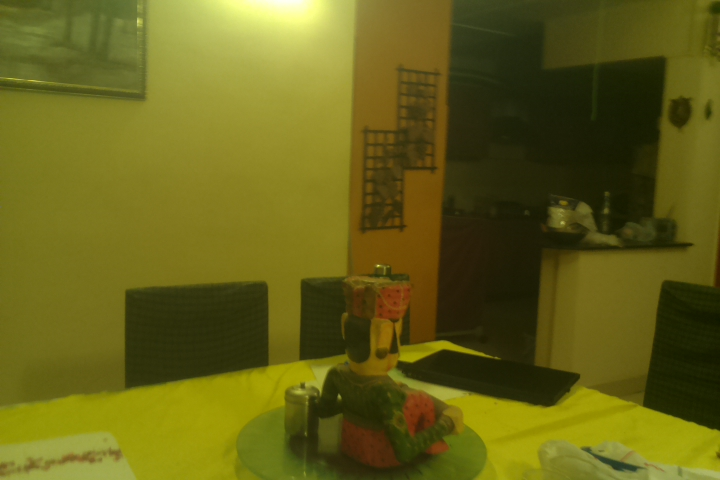
\includegraphics[width = 2.6cm]{pano3d/3d3.jpg}
  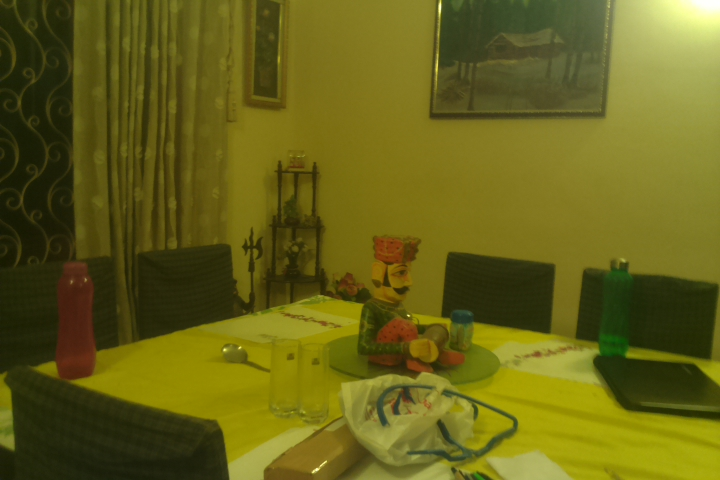
\includegraphics[width = 2.6cm]{pano3d/3d4.jpg}
  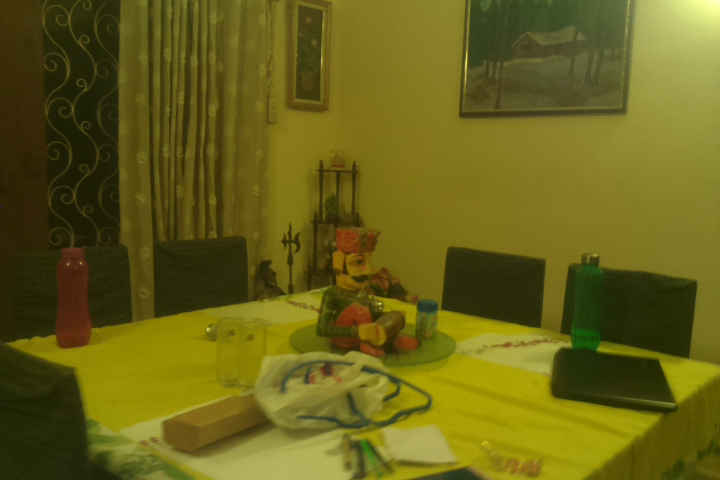
\includegraphics[width = 2.6cm]{pano3d/3d5.jpg}
  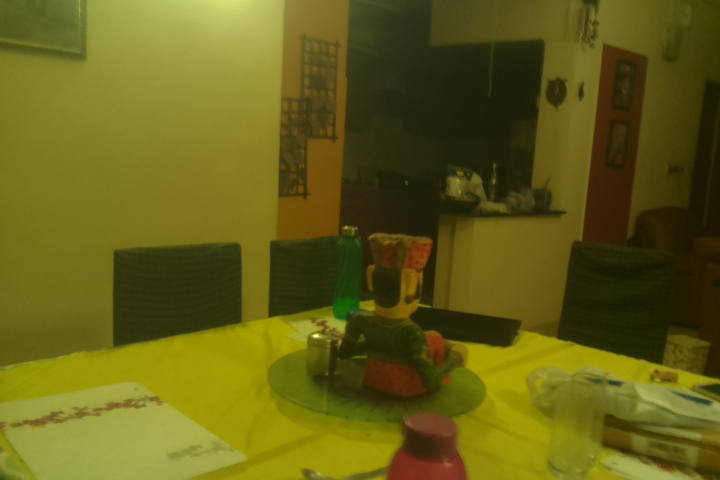
\includegraphics[width = 2.6cm]{pano3d/3d2.jpg}
  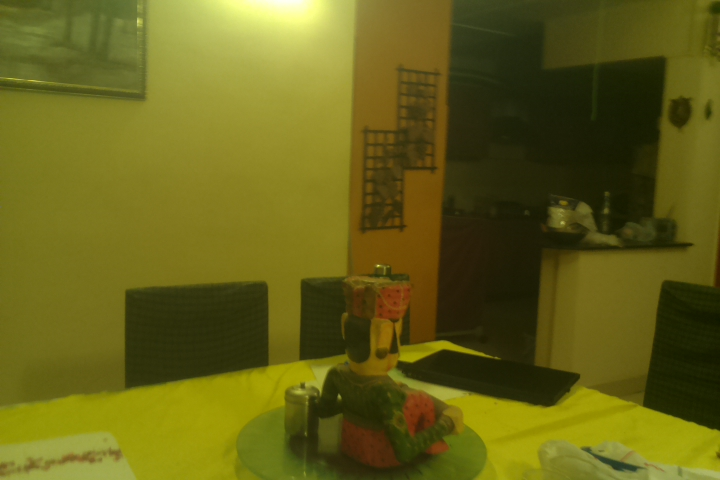
\includegraphics[width = 2.6cm]{pano3d/3d3.jpg}
  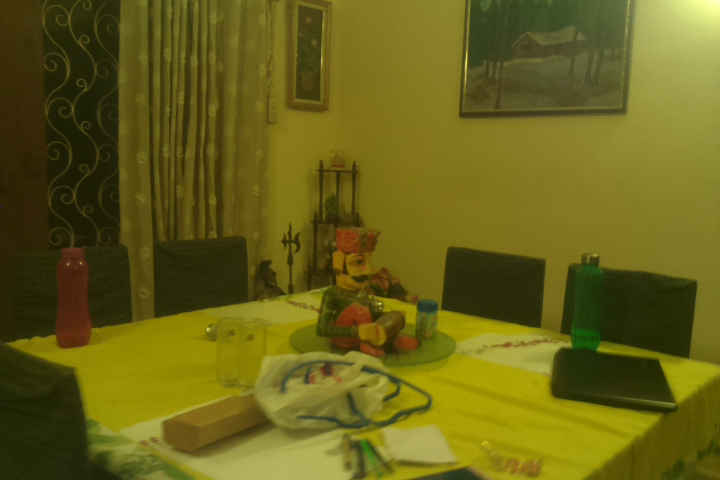
\includegraphics[width = 2.6cm]{pano3d/3d5.jpg}
  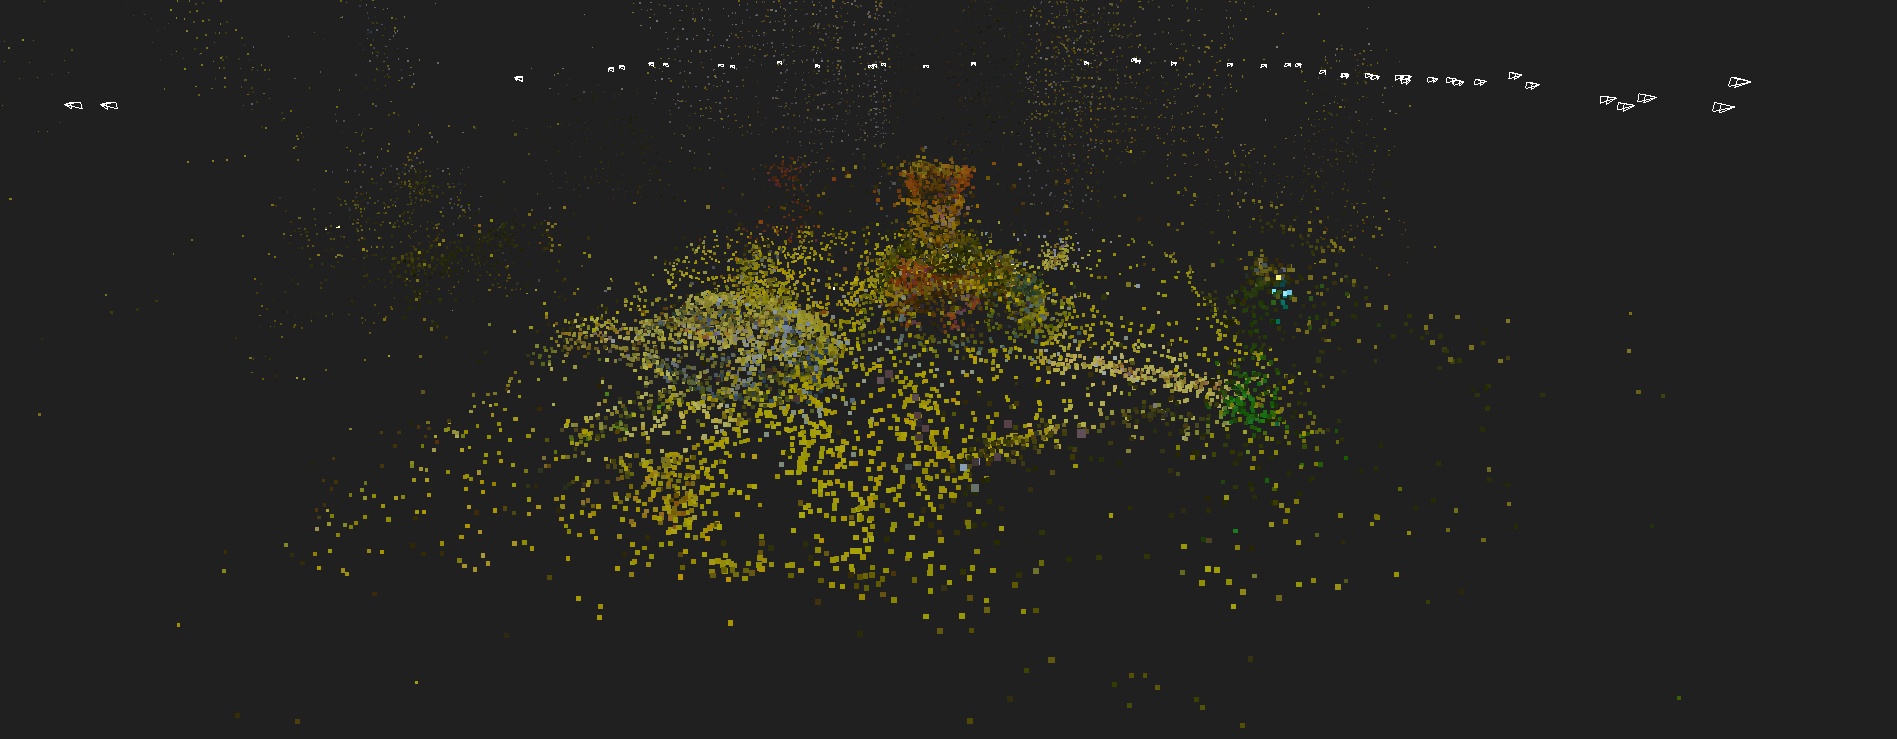
\includegraphics[width = 15cm]{pano3d/3d.png}
  \caption{3D Reconstruction of test images where colored point cloud is rendered on the browser which can be inspected closer.}
  \label{recon}	
\end{figure}

\pagebreak
\subsection{Android App}
The Android App is used to control all the operations on the quadcopter. It implements a virtual Joystick interface for easy user-interaction.
The interface consists of two joysticks, buttons to start the quadcopter program, enable camera mode, dynamically alter x and y trim values and a text box for feeding in the IP address of the RPi.
\newline
\newline
The two joysticks - left and right are for for altitude control and motor control respectively. The user can swipe upwards and downwards on the left joystick to increase and decrease the height of the quadcopter.  Similarly, the user can swipe in all directions on the right joystick to control the speed of individual motors depending on the distance from the center of the joystick. 
\newline
\newline
The x and y trim values can be dynamically changed using the app. These values are used to add bias to the quadcopter and control its stability. 
The camera button can enable or disable camera mode on the quadcopter. Enabling it allows the RPi camera to begin shooting pictures with an interval of 1 second while disabling it stops the camera program.
\newline
\newline
Using an Android app to remotely control UAVs is a level up from traditional RC controllers as it allows users greater flexibility. Users can now control many more aspects of the quadcopter apart from height and orientation such as camera control and bias using a simple and attractive user interface.
\newline
The next chapter deals with the Results and Evaluation of test cases.
\begin{figure}[H]
  \centering
  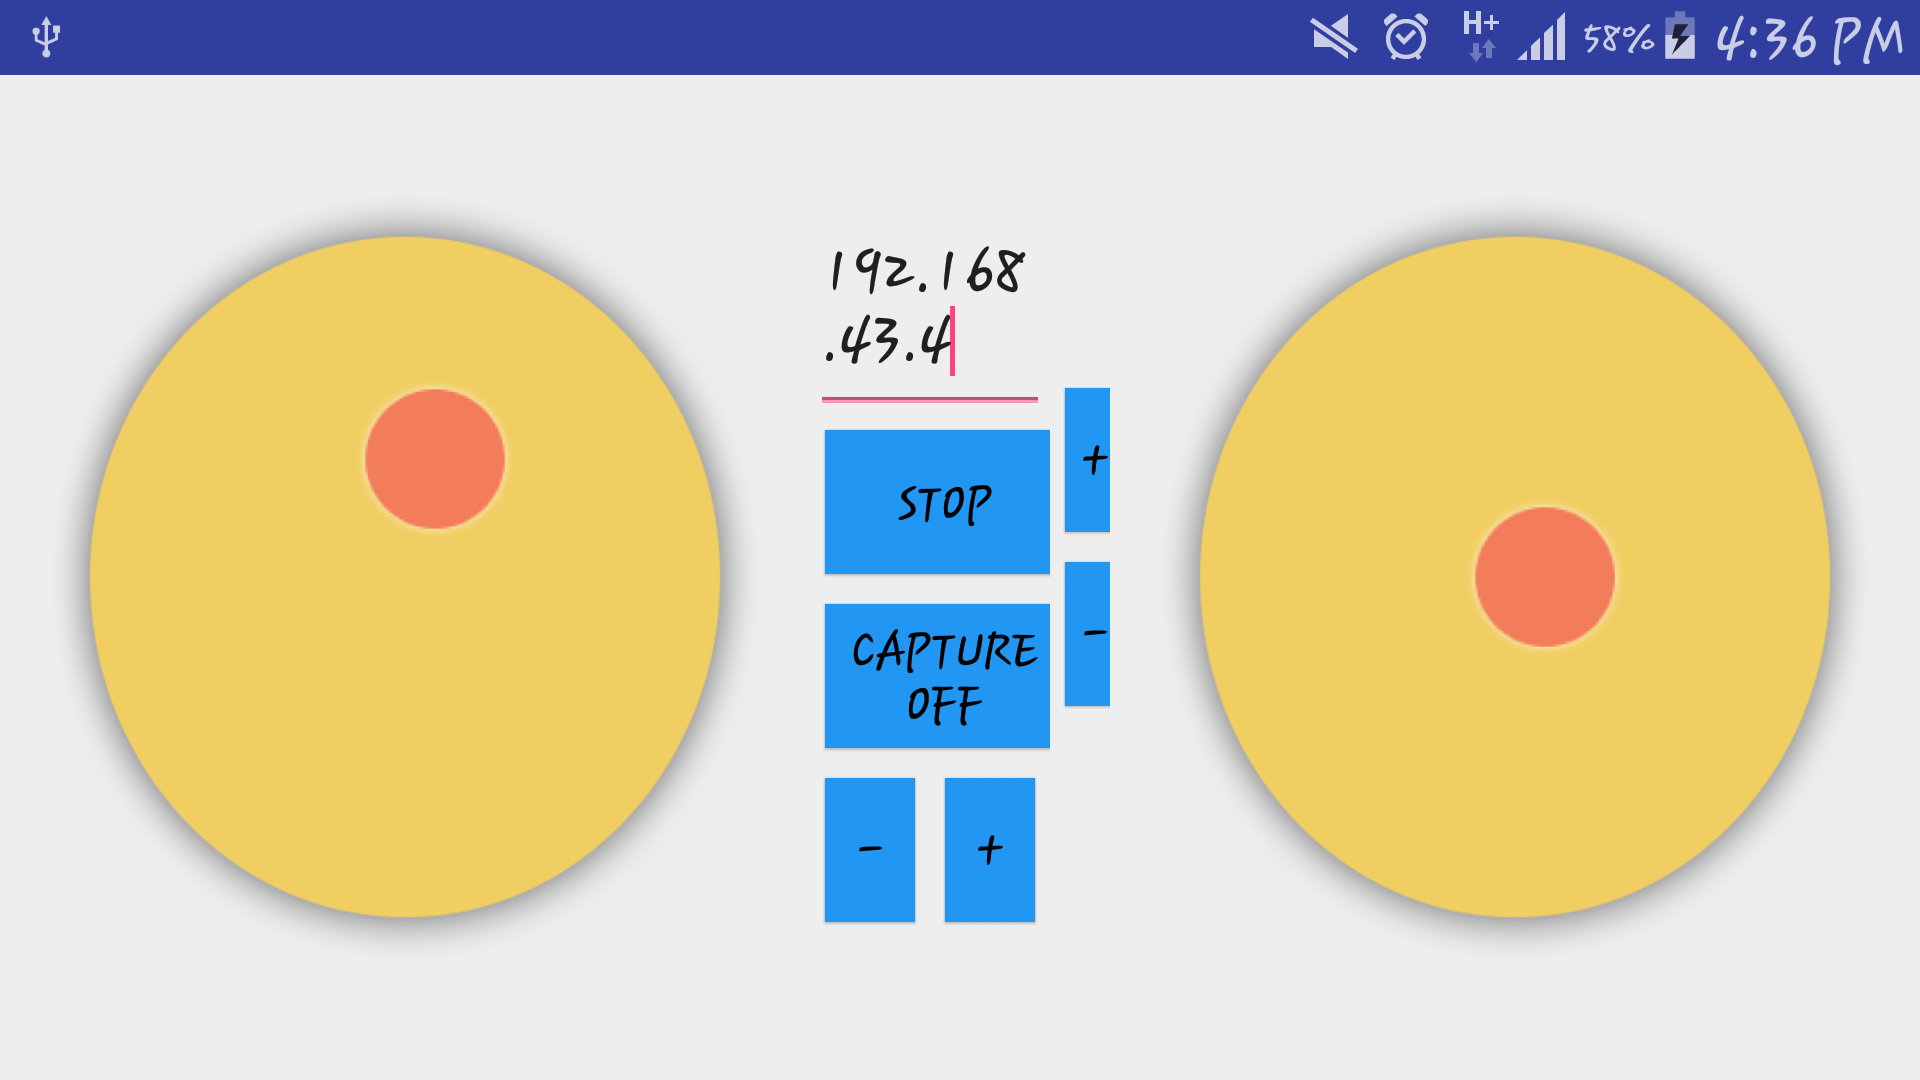
\includegraphics[width = 15cm]{app.png}
  \caption{Android App Joystick Interface}
  \label{app} 
\end{figure}

\section{Overall Component Diagram}
\begin{figure}[H]
  \centering
  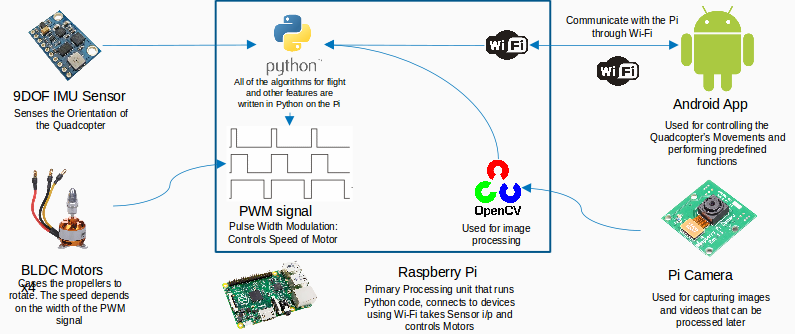
\includegraphics[width = 15cm,height = 9cm]{software_comp.png}
  \caption{Overall Hardware and Software Component Diagram describing the flow of execution}
  \label{Software Flow}	
\end{figure}

